\section{Panel Data in the Marketing Analytics Ecosystem}
\label{sec:marketing-ecosystem}

Marketing organisations measure effectiveness through four broad approaches, each with distinct strengths and limitations.  Understanding where panel methods fit is critical for selecting the appropriate tool.

Attribution modelling is ubiquitous in digital marketing, but as noted in Section~\ref{sec:measurement-crisis} it remains observational and platform-specific. It reports which touchpoints precede conversions rather than counterfactuals, and often omits spillovers. We use it for optimisation, not for causal effects.

Marketing mix modelling (MMM) can be estimated using aggregate time series or panels that include adstock and saturation. As discussed earlier, aggregate time-series MMM faces identification and spillover challenges and struggles with discrete interventions. Panel MMMs are complementary; we contrast them with the common aggregate implementation.

The third pillar, geo-experiments, represents the gold standard of causal inference. By randomising treatment across geographic markets---designated market areas, stores, regions---firms generate clean variation in marketing actions that is, by design, uncorrelated with potential outcomes. Geo-experiments are particularly valuable when spillovers are localised within markets (internal to treatment or control clusters) and when the intervention can be implemented at market level. Platforms such as Meta, Google, and Amazon now provide tools for large-scale geo-experiments, lowering adoption barriers. Nevertheless, geo-experiments face practical limitations: spillovers across geographies can contaminate estimates, small numbers of clusters limit statistical power, short durations may miss long-run effects, and the cost and complexity of randomised rollouts can be prohibitive.

Panel data methods constitute the fourth pillar. The modern approaches that are the focus of this book apply quasi-experimental identification strategies to observational data, exploiting natural variation in the timing, location, or intensity of marketing actions to estimate causal effects. Unlike attribution models, panel methods explicitly model counterfactual outcomes under control conditions while making testable assumptions about unobserved confounding. Unlike typical aggregate time-series MMM implementations, panel methods can isolate discrete interventions, accommodate staggered adoption, and incorporate unit and time heterogeneity using fixed effects or factor structures. Unlike geo-experiments, panel methods do not require randomisation, enabling analysis of historical data, long-run effects, and settings where randomisation is infeasible. In practice, MMM and panel designs often overlap---for example, panel MMM with adstock and saturation fitted under a design-based identification strategy.

Panel causal designs require design-specific assumptions, not a one-size-fits-all condition. Some methods — difference-in-differences, event studies, interactive fixed effects (Chapters~\ref{ch:did}, \ref{ch:event}, \ref{ch:factor}, \ref{ch:advanced-matrix}) — rely on some form of parallel evolution across treated and control units. Others — synthetic control and its variants (Chapters~\ref{ch:sc}, \ref{ch:generalized-sc}) — substitute strong pre-treatment fit for parallel trends assumptions. Still others — instrumental variables, regression discontinuity, dynamic panel GMM — require entirely different identifying structures: relevance and exclusion, continuity at a threshold, or moment conditions with specific serial correlation patterns. Throughout, we signpost assumptions and diagnostics in Chapters~\ref{ch:did}--\ref{ch:spillovers} and \ref{ch:inference}.

How should a practitioner decide which tool to use? The data structure drives the choice. Without repeated observations on the same units over time, panel methods are off the table. When repeated observations exist, randomisation remains the first-best option. Experiments provide clean identification, though panel methods still add value by controlling for pre-treatment imbalances, quantifying heterogeneity, and extending short-term experimental results through longer observational follow-up. 

When randomisation is infeasible, the structure of treatment variation guides method selection. Discrete interventions at specific points in time call for difference-in-differences or synthetic control methods (Chapters \ref{ch:did}, \ref{ch:event}, \ref{ch:sc}, \ref{ch:generalized-sc}). Treatments that vary smoothly over time or across units without clear pre-post divides suit factor models and matrix completion methods (Chapter \ref{ch:factor}). Spillovers and interference demand methods that explicitly model network or geographic linkages (Chapter \ref{ch:spillovers}). High-dimensional covariates or heterogeneous treatment effects benefit from machine learning integration (Chapters \ref{ch:ml-nuisance}, \ref{ch:high-dim}).

Figure~\ref{fig:ecosystem} visualises these four pillars and their relationships. The overlapping circles represent not competition but complementarity. Where circles intersect, we find opportunities for triangulation: randomised experiments can validate panel-based estimates and calibrate MMM parameters; panel methods can extend short-run experimental results to longer horizons and provide causal interpretations of attribution metrics; marketing mix models can guide channel selection for deeper causal analysis; attribution models can flag segments warranting experimental scrutiny.

At the centre, where all four approaches converge, lies triangulation: multiple methods with different assumptions collectively build a more robust case for causality than any single method alone. The figure also highlights distinct timelines---experiments measure effects over days or weeks, panel methods track months or years, MMMs aggregate weeks or quarters, attribution provides real-time feedback. Understanding these complementarities is essential for coherent measurement strategy.

\begin{figure}[htbp]
\centering
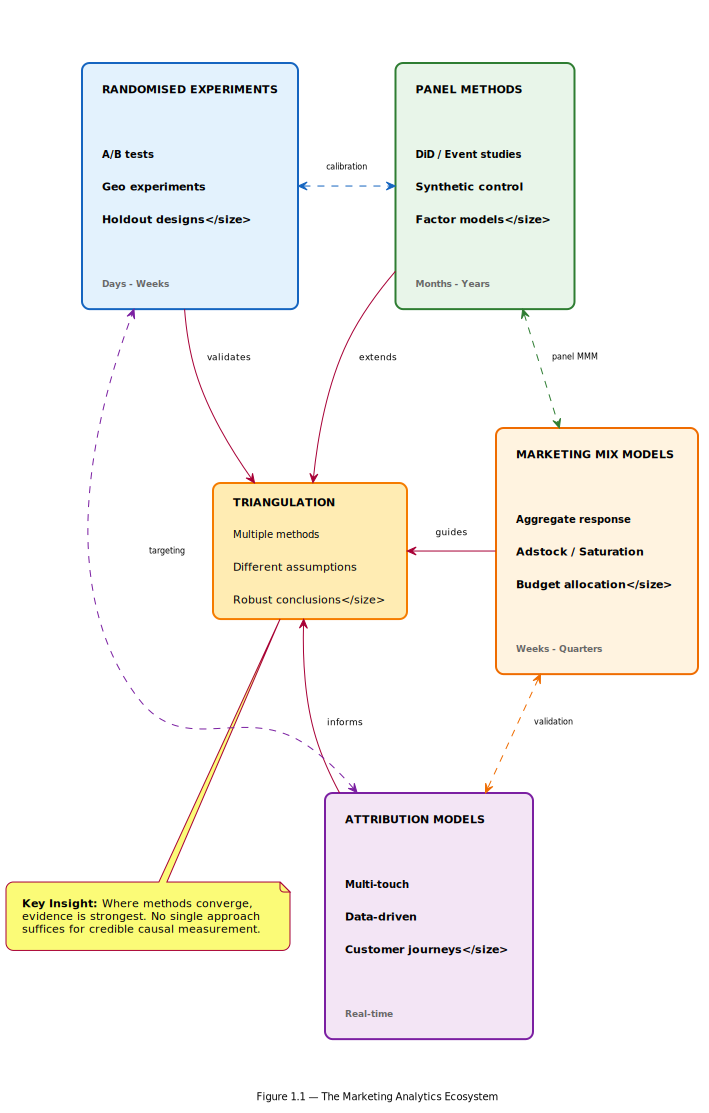
\includegraphics[width=0.7\textwidth]{images/ecosystem.png}
\caption{The Marketing Analytics Ecosystem: Experiments, Panels, MMM, and Attribution}
\label{fig:ecosystem}
\end{figure}

MMM and panel methods are not mutually exclusive. Many workflows combine MMM-style transforms (adstock, saturation) with design-based identification in panels (DiD, SC, IV). Panel MMMs are natural when you have multi-market or store-level data, and design-based logic strengthens identification. Factor-augmented panels (Chapters~\ref{ch:factor}, \ref{ch:advanced-matrix}) and instrumental variables (Chapters~\ref{ch:frameworks}, \ref{ch:inference}) further bridge modelling and design.

Today's methods did not emerge fully formed. They reflect decades of intellectual development responding to new data, computational capabilities, and substantive challenges. Figure~\ref{fig:timeline} depicts this evolution.

The 1980s and 1990s were dominated by two-way fixed effects and random effects models controlling for time-invariant unobservables. The design-based revolution of the 2000s brought synthetic control methods \citep{abadie2003economic,abadie2010synthetic} and renewed focus on difference-in-differences with explicit parallel trends assumptions. The late 2010s saw the discovery of negative weighting in staggered TWFE designs \citep{goodman2021difference,dechaisemartin2020two}, sparking heterogeneity-robust estimators that aggregate cohort-specific effects without using previously treated units as controls.

Recognition that parallel trends in levels may be too restrictive motivated synthetic control methods matching on pre-treatment trajectories. The proliferation of high-dimensional data---rich customer covariates, detailed competitor actions, granular geographic variation---prompted machine learning integration for flexible control and heterogeneous effect estimation. This timeline demonstrates the iterative, self-correcting nature of methodological progress. Today's methods will be refined or replaced as new challenges arise. The marketing applications driving this book---loyalty programmes, advertising campaigns, platform expansions---have played an important role, providing both motivation for new methods and empirical testing grounds where strengths and limitations can be identified.

\begin{figure}[htbp]
\centering
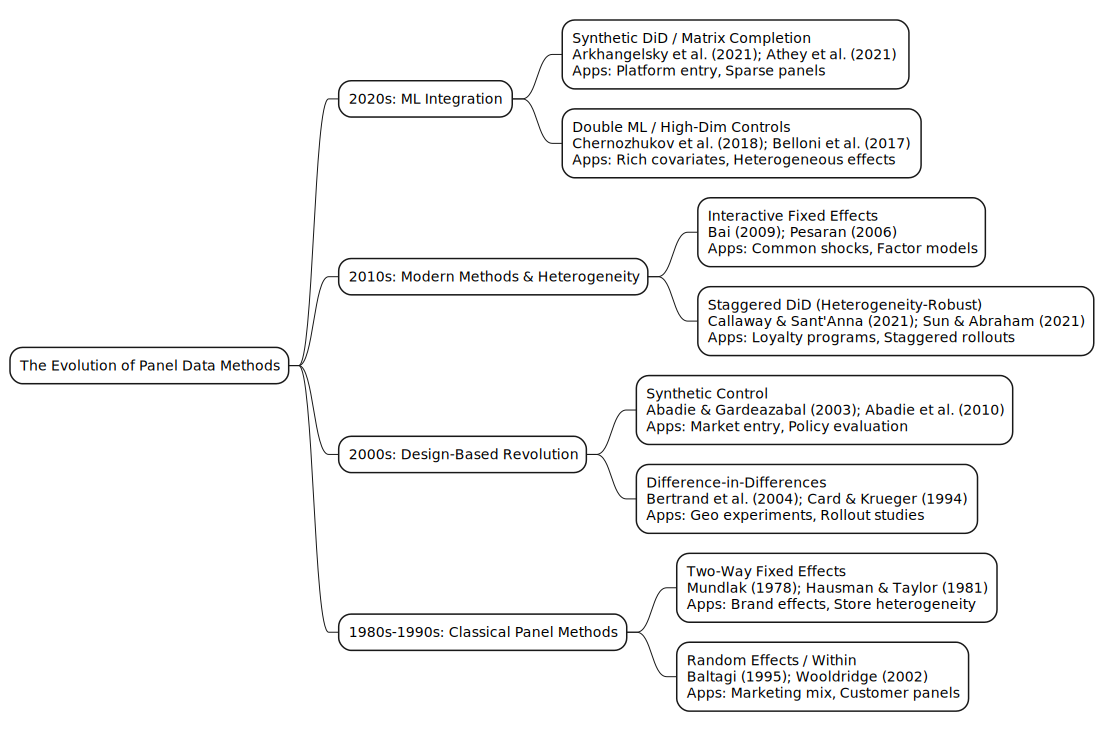
\includegraphics[width=0.95\textwidth]{images/timeline.png}
\caption{Timeline of Panel Data Methods: From TWFE to Modern Heterogeneity-Robust and ML-Integrated Approaches}
\label{fig:timeline}
\end{figure}

The aims of this book grew out of several converging developments rather than a single influence. A sequence of methodological breakthroughs in causal inference for panel data, together with a rapidly expanding applied literature, has made it possible to study marketing interventions with far greater rigour than traditional time-series or attribution approaches allow. At the same time, much of the marketing analytics discourse has drifted toward predictive machine learning, often with only loose connections to identification and design. This book attempts to recentre the discussion on causal structure and research design, while still drawing on modern tools where they genuinely strengthen empirical work.

Within this landscape, \citet{arkhangelsky2024causal} provides a rigorous synthesis of modern causal panel methods. We build on similar foundations but with different emphasis: marketing-specific issues---attribution challenges, algorithmic confounding, applications in loyalty programmes and advertising---that receive limited attention in econometrics texts; machine learning as a supporting tool for identification rather than stand-alone prediction; and a practitioner orientation emphasising intuition, diagnostics, and method selection over formal proofs, while maintaining technical precision in assumptions and identification.
